% !TEX root = ../thesis.tex
%=========================================================
\chapter{Practical Notes on Sample Fabrication}
\label{appendix:sample-fabrication}
%=========================================================

    This section collects practical notes from the laboratory that complement the conceptual description in the main text. It is not intended as a fully standardized protocol. Instead, it documents the small but critical steps, common pitfalls, and empirically useful habits that make reliable sample preparation more likely.


    \subsubsection*{Wafer Preparation}
        Start with a \qty{300}{\micro\meter} thick bronze wafer, which is typically covered by a protective foil. To remove this foil without damaging the wafer, cool the wafer in liquid nitrogen and then gently peel off the brittle fragments. This method has proven effective and largely non-destructive. The wafer is then polished. For this purpose, attach a polishing head made of sewn cotton cloth to a drill and use aluminum oxide from a white polishing compound block as the abrasive. The polishing head should be well moistened, preferably soaked, with a solvent such as ethanol or IPA. Fix the wafer to a smooth milled steel block using double-sided adhesive tape\footnote{e.g. Tesa Universal}, taking care that no tape protrudes beyond the wafer edge. During polishing, move the polishing head from top to bottom so that debris generated in the process is less likely to settle back onto the wafer surface. Rotate the steel block periodically, since the lower part of the wafer is generally easier to polish uniformly. Polishing is complete once the entire surface shows a homogeneous mirror-like finish. To detach the wafer from the steel block, cool it again in liquid nitrogen. For cleaning, rinse the wafer first with acetone and then with IPA, ensuring that the acetone is removed completely before switching solvents. Finally, dry the wafer with pressurized nitrogen while the IPA is still wet in order to avoid residue formation. \cite{oberg_machinerys_2000}
        
        An alternative polishing method uses sandpaper with progressively finer grit on a glass slide, as described by Patrick Raif \cite{raif_fabrication_2023}. It is better suited to reducing long-range surface variations, but it is also considerably more time-consuming and was therefore not used routinely.

        Next, prepare the spin coater, the polyamide (PA), and the vacuum oven. The PA is pre-portioned into small crimp-seal vials to minimize moisture exposure and to reduce the time required for warming. Remove one vial from the freezer and allow it to reach room temperature while preheating the convection oven to \qty{135}{\degreeCelsius}. Line the inside of the spin coater with aluminum foil and verify that the vacuum oven is operational and open.

        To remove adsorbed water, place the wafer on a hot plate at \qty{100}{\degreeCelsius} for at least one minute. For reliable adhesion to the \qty{1}{\inch} chuck, apply a layer of parafilm and bend it securely around the chuck edge. Then make five small holes in the parafilm using a syringe: one in the center and one near the edge in each cardinal direction. Allow the wafer to cool to room temperature before centering it on the chuck, and only then switch on the vacuum pump. Before dispensing the PA, it is advisable to run the spin-coating program once as a quick check that the wafer is held securely. This is particularly important for larger wafers, where insufficient adhesion may not be immediately obvious.
        
        Blow the wafer dry with nitrogen to remove residual dust. Pour the PA onto the wafer so that roughly 90\,\% of the surface is covered, taking care to avoid trapped air bubbles. If bubbles remain, move or burst them carefully with a syringe without scratching the wafer. The spin-coating program consists of an initial spread step at \qty{300}{\rpm} for \qty{30}{\second} followed by a final spin step at \qty{5000}{\rpm} for \qty{90}{\second}. Immediately afterward, transfer the wafer to the convection oven for a \qty{5}{\minute} soft bake at \qty{135}{\degreeCelsius}. The hard bake is then performed in the vacuum oven using a programmed cycle that ramps to \qty{400}{\degreeCelsius}, holds for \qty{30}{\minute}, and cools back to room temperature over several hours. Detailed instructions and the corresponding temperature profile are given in Ref.~\cite{raif_fabrication_2023}. In practice, starting the bake immediately after spin coating has been found to improve reproducibility.
        
        The application of the EL11 and A4 resist layers follows the same general workflow, but the individual spin and baking parameters differ. In this case, aluminum foil inside the spin coater is unnecessary because these resists can be removed easily with acetone. The age of the resist should be checked before use, since prolonged storage can noticeably degrade performance. In particular, EL11 is first followed by its soft-bake step. After the A4 layer is applied, the subsequent A4 baking step also hard-bakes the underlying EL11 layer. The relevant process parameters in this subsection follow Table \ref{tab:methods:sample_parameter}.

        The wafer is then cut into smaller pieces of 3\,$\times$\,\qty{8}{\milli\meter} using a custom shear-sheet cutter equipped with \qty{3}{\milli\meter} and \qty{18}{\milli\meter} spacers. Before cutting, clean the cutting edges thoroughly with IPA to reduce contamination and to maintain clean cuts. Samples taken from the outer wafer region are more likely to show thickness variations in the PI and resist layers. For reproducible fabrication, pieces from the central region of the wafer are therefore preferred. Edge-related thickness variations can affect the dose required during electron-beam lithography. After cutting, store the samples in a chip tray\footnote{e.g. Entegris} for safe handling.

    \subsubsection*{Electron beam lithography}
        The next step is electron-beam lithography (EBL) using the Crossbeam system. Begin by measuring the beam current with the jig containing the Faraday cup. A position list in the Zeiss software is helpful for locating the Faraday cup quickly. For reliable operation, the working distance should be kept as close as possible to \qty{5.00}{\milli\meter}. Since the beam current may require some time to stabilize, it is often useful either to wait before measuring or to return later and repeat the check.

        Accurate horizontal alignment of the sample is essential for exposure. The alignment tools in the Focused Ion Beam (FIB) toolbox simplify this step. A practical approach is to zoom out to the maximum field of view and use the upper-right corner of the sample together with the farthest left sample edge for the initial alignment. This is usually sufficient to correct the dominant angular misalignment. Additional refinement within Elphy Plus is possible, but in practice it rarely improves the final angular alignment once the sample is mounted in the cryostat.

        Next, focus the beam in the upper-right corner of the sample. Use the wobble function to center the beam in the aperture and minimize astigmatism with the \textit{x}- and \textit{y}-stigmators. Once the beam is well focused, check the current again at the Faraday cup. For the \qty{30}{\micro\meter} aperture in high-current mode, the beam current should be about \qty{0.5}{\nano\ampere}. This setting is used for the small high-resolution structures. For the \qty{120}{\micro\meter} aperture, which is used for the \qty{1000}{\micro\meter} writing fields, the exact current is less critical because the larger leads tolerate moderate underexposure. In practice, a slight underexposure in these larger fields can even reduce writing time without compromising the result. The beam current for the \qty{120}{\micro\meter} aperture in high-current mode is typically around \qty{5}{\nano\ampere}. Perform a final focusing step at the central position along the upper sample edge. A dirt particle on the resist is often useful as a focusing aid. At this stage, confirm once more that the working distance is \qty{5.00(1)}{\milli\meter} and that the beam shift is set to zero.

        Before starting the exposure, note the current time. Since the design layout includes a timestamp, this provides a convenient way to match laboratory notes to the physical sample. If the measured beam current differs from earlier sessions, recalculate the settling time for the \qty{100}{\micro\meter} field accordingly. The executed position list in Elphy Plus then locates the writing fields automatically, applies the corresponding settings, and writes the design. Stitching between adjacent writing fields is enforced by overlapping their nominal positions by \qty{100}{\micro\meter}.

        In practice, it is advantageous to keep the written design as simple as possible and to avoid an unnecessarily large number of polygons. This reduces writing overhead and makes the exposure procedure more robust. In addition, contamination dots were deliberately avoided as focusing markers. Instead, the combination of high-current mode and the \qty{30}{\micro\meter} aperture proved sufficient for reliable focusing because it provides a comparatively large depth of focus. The drawback is that very low exposure doses are no longer readily accessible, but this was not a practical limitation for the structures used here.
        
        Repeat the full alignment, focusing, and writing sequence for the remaining samples until a batch of roughly four to five samples has been completed.

        If several weeks have passed since the previous EBL session, it is advisable to verify the alignment between the \qty{100}{\micro\meter} and \qty{1000}{\micro\meter} writing fields before exposing the first sample. A simple check is to expose one \qty{100}{\micro\meter} field together with a neighboring \qty{1000}{\micro\meter} field in the upper-right corner of a sample. The exposed resist appears visibly different from the unexposed surroundings and can therefore be used to judge the relative alignment. Prolonged observation should be avoided, however, since the resist can be exposed unintentionally and lose contrast. If misalignment is found, adjust the settings accordingly. For example, if the \qty{100}{\micro\meter} field is shifted to the left, correct \textit{U} by --$\Delta$\textit{X}; if it is shifted upward, correct \textit{V} by --$\Delta$\textit{Y}. Repeat the test until the alignment is satisfactory.

        After exposure, the samples are developed. Prepare a crimp-seal vial containing a mixture of one part MIBK and three parts IPA, and prepare one additional vial of pure IPA for each sample. Immerse the sample in the MIBK/IPA developer for \qty{25}{\second} while gently swirling the vial to maintain uniform development. Then transfer the sample immediately into pure IPA and continue swirling. The developer can be reused for all samples in the same batch, whereas fresh IPA should be used for each individual sample. Leave the sample in IPA for \qty{60}{\second}, then remove it and dry it carefully with a stream of nitrogen. During the full process, hold the sample securely with tweezers to avoid accidental dropping during waiting or transfer steps. Finally, inspect the developed structures under a light microscope to verify that the pattern is complete and free of obvious defects.

    \subsubsection*{Shadow Evaporation}
        To begin shadow evaporation, place the sample holder on a hot plate at \qty{100}{\degreeCelsius} for a few minutes in order to remove adsorbed water. This step improves the vacuum noticeably. Check the sample orientation carefully so that the shadow evaporation proceeds in the intended direction. For best results, load the sample into the load lock and pump it overnight, or longer if possible, before starting the deposition sequence.

        Once the vacuum is satisfactory, transfer the sample holder into the main chamber for the first evaporation. Using electron-beam evaporation, deposit \qty{60}{\nano\meter} of aluminum at an angle of \qty{4}{\degree}. Heat the aluminum gradually over approximately \qtyrange{5}{10}{\minute} to avoid stressing the crucible and to promote stable evaporation. The crucible should contain a sufficient amount of aluminum; in practice, one to three pellets per evaporation are typically adequate.

        After the first evaporation, transfer the sample back into the load lock and close the pumping line. Introduce pure oxygen until a pressure of \qty{3.0(2)}{\milli\barunit} is reached and oxidize the sample for \qty{3}{\minute}. To terminate the oxidation, reopen the pumping line. In order to recover a vacuum on the order of 10$^\text{--6}$\,mbar afterward, it is important that the oxygen feed line itself has been evacuated thoroughly.

        Once the load lock vacuum has recovered, transfer the sample back into the main chamber for the second evaporation. Deposit \qty{100}{\nano\meter} of aluminum at an angle of \qty{34}{\degree} to complete the shadow-evaporation sequence.

        A smooth aluminum surface is desirable for forming a well-defined Al$_\text{2}$O$_\text{3}$ layer. In practice, however, the deposited aluminum often showed a large number of dimples. Several measures were tested in an attempt to reduce them, but no decisive remedy was identified. There was some indication that higher evaporation rates, in particular values above 4\,\AA/s, may reduce the number of dimples, although the effect was not statistically convincing. Somewhat contrary to earlier expectations, a less extreme vacuum or a shorter time between the last vacuum break and the evaporation occasionally appeared to improve the surface. One possible interpretation is that a very clean sample mainly suppresses desorption of water or other contaminants during deposition, whereas a less ideal chamber condition may influence nucleation in a way that incidentally smooths the film. Since the observed differences remained small, the issue was not pursued further.

        Lift-off is performed by placing the sample in a crimp-seal vial filled with pure acetone and heating it on a hot plate at about \qty{60}{\degreeCelsius} for \qtyrange{1}{3}{\hour}. Afterward, use a pipette to agitate the acetone carefully until all visible metal flakes have detached. Rinse the sample with IPA and dry it with nitrogen.

    \subsubsection*{Plasma Etching}
        The penultimate fabrication step is plasma etching using the PlasmaPro 80 ICP RIE system by Oxford. Although this tool is not designed specifically for highly homogeneous etching, it can be operated in a regime that gives sufficiently uniform results by combining low table RF power with elevated pressure. An ignition step is used first to stabilize the plasma before switching to the less stable regime that favors homogeneous etching. The sample temperature is particularly important for obtaining the desired undercut. A table temperature of \qty{100}{\degreeCelsius} proved to be a good compromise: it produces a sufficient undercut while keeping the etch slow enough to control the depth reliably. The process parameters that gave the best results are listed in Table \ref{tab:methods:rie_parameter}.
        \begin{table}
            \centering
            \caption{RIE recipe \texttt{MCBJ SSET v5 @ 100C}}
            \label{tab:methods:rie_parameter}
            \vspace{1em}
            \begin{tabular}{llll}
                \hline
                Parameter       & Stabilization         & Ignition      & Etching  \\
                \\\hline
                Process time    & \qty{5}{\minute}                & \qty{5}{\second}          & \qty{30}{\minute}       \\
                Table heater    & \qty{100}{\degreeCelsius}   & -             & -             \\
                Oxygen flow     & \qty{50}{\sccm}           & -             & -             \\
    
                Pressure        & \qty{100}{\milli\torr} & ramp & \qty{250}{\milli\torr} \\
    
                \\\hline
                Table RF &&&\\
                Power Demand            & - & \qty{20(5)}{\watt}              & \qty{3(5)}{\watt} \\
                Max Reflected Power     & - & \qty{5}{\watt}                  & \qty{2}{\watt} \\
                Tolerance Time          & - & \qty{7}{\second}                  & - \\
                Min dc bias             & - & \qty{1}{\volt}                  & - \\
                AMU (C1, C2)            & - & (41\,\%, 23\,\%)      & - \\
    
                \\\hline
                ICP RF &&&\\
                Power Demand            & - & \qty{400(50)}{\watt}            & - \\
                Max Reflected Power     & - & \qty{100}{\watt}                & - \\
                Tolerance Time          & - & \qty{10}{\second}                 & - \\
                AMU (C1, C2)            & - & (64\,\%, 39\,\%)      & - \\
                
            \end{tabular}
        \end{table}
        
        A laser interferometer is used to monitor the etched depth. For this purpose, choose a spot on the sample without metal structures where the reflected intensity is as large as possible without reaching saturation. 
        
        \begin{wrapfigure}[13]{r}{0.4\textwidth}
            \captionsetup{format=plain}%
            \centering
            \vspace{-1em}
            \thesisplot{methods/sample}{rie}
            \caption{Recorded laser intensity $I_{\mathrm{Laser}}(t)$ during plasma etching. The process is terminated after approximately 2.8 periods, corresponding to the target etch depth.}
            \label{fig:methods:rie}
        \end{wrapfigure}
        During the etch, the signal follows an approximately cosine-like oscillation that can be used to estimate the removed thickness. The required number of periods $m$ depends on the laser wavelength $\lambda=\qty{632.8}{\nano\meter}$, the target depth $d=\qty{500}{\nano\meter}$, and the refractive index $n=1.81$\footnote{Fujifilm Electronic Materials U.S.A., Inc., \texttt{Polyamic Acid. Durimide 100}}. For the present process, the target value is
        \begin{align}
            m = \frac{2 \cdot n \cdot d}{\lambda} = \frac{2 \cdot 1.81 \cdot \qty{500}{\nano\meter}}{\qty{632.8}{\nano\meter}} = 2.86
        \end{align}
        periods. An example of the recorded laser intensity during etching is shown in Fig.~\ref{fig:methods:rie}.
        
        Since the etch rate varies noticeably from sample to sample, each sample should ideally be etched individually.

    \subsubsection*{Electrical contacting}
        Electrical contacting is one of the most delicate steps in the entire fabrication sequence. Many otherwise successful samples are lost at this stage, so patience and a calm working setup are more important than speed. In practice, it is usually better to contact fewer samples carefully than to rush several samples in one session.

        Good working conditions matter. Stable hand positioning, appropriate lighting, and a comfortable bench height all make the process significantly easier. A setup that allows the operator to sit close to the sample while keeping both hands supported is particularly helpful. It is also worth minimizing avoidable sources of hand tremor before starting.

        To fix the sample, adhesive strips\footnote{e.g. tesafilm\textregistered\ standard by Tesa} are used on a copper plate. This arrangement keeps the sample in place while still allowing some freedom to reposition the plate. Prepare \qty{90}{\micro\meter} insulated copper wires soldered to post connectors in advance. The wire ends should be stripped, and the bias-line wires may be twisted. The wires should be kept as short as practical; typically, $\qtyrange{4}{5}{\centi\meter}$ is sufficient. The rear part of each post connector should be insulated with a varnish\footnote{e.g. GE Low Temperature Varnish (59-C5-101) by Oxford Instruments}.

        \begin{wrapfigure}[14]{r}{0.4\textwidth}
            \captionsetup{format=plain}%
            \centering
            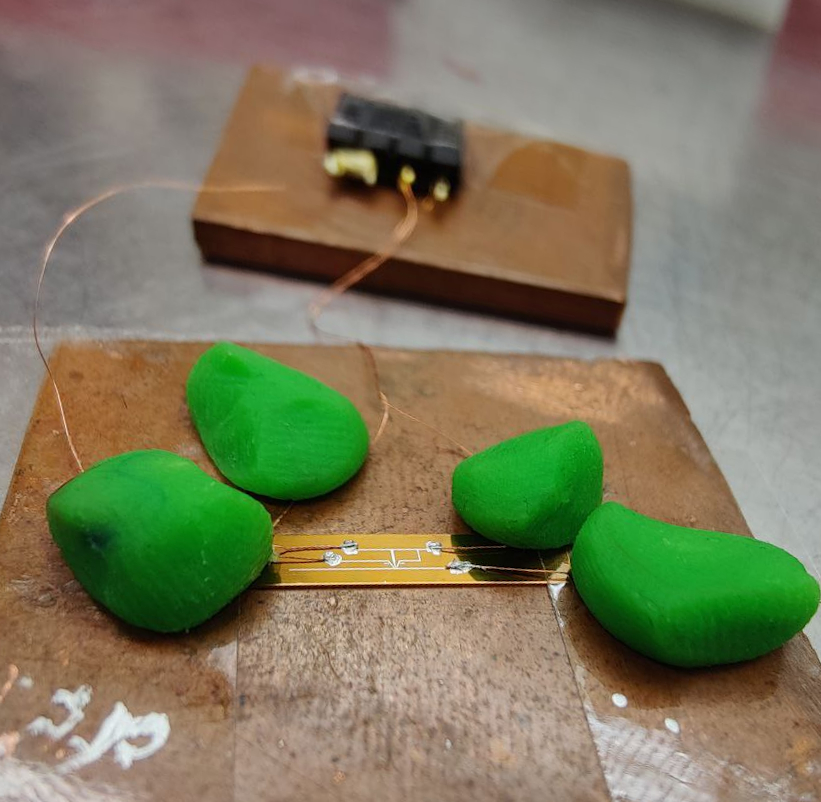
\includegraphics[width=.4\textwidth]{methods/sample/contacting/contacting.jpg}
            \caption{Example of a contacted sample, before adding strain relief.}
            \label{fig:methods:contacting}
        \end{wrapfigure}
        Position the wire ends on the sample pads with the help of play dough. Then, using a sharpened toothpick, apply a small amount of silver paste to connect each wire to its pad. The viscosity of the silver paste is critical: if it is too fluid, shorts can form; if it is too viscous, it tends to remain on the toothpick instead of wetting the pad properly. In practice, using paste collected from the lid after shaking the bottle works well. Only a very small amount should be transferred, just enough to wet the pad. Afterward, apply two-component epoxy as strain relief for the wires. Here as well, the viscosity is important. If the epoxy is used too soon after mixing, it continues to flow and may spread into unwanted areas. Since the interaction between epoxy and silver paste is not fully understood, the two materials should be kept separate as much as possible. A useful approach is to test the epoxy on small trial dots and wait until it reaches a suitable consistency before applying it to the sample. The two sides of the sample are best glued separately, since the useful working window is fairly short.
        
        After the sample has been mounted in the cryostat, the final step is to scratch the shorting bridge with an engraving tool. During this step, and also while closing the radiation shields, proper grounding is essential. Wearing a grounding bracelet is recommended. In dry conditions, additional precautions such as increasing the ambient humidity can further reduce the risk of electrostatic discharge.

    \newpage
    \subsubsection*{Summary of key process parameters}
        \begin{table}[!h]
            \centering
            \caption{Key process parameters used for sample preparation.}
            \label{tab:methods:sample_parameter}
            \vspace{1em}
            \begin{tabular}{ll}
                \hline
                Sacrificial layer   & Durimide 115A\\
                Spinning            & spread cycle: \qty{300}{\rpm} for \qty{30}{\second}\\
                                    & spin cycle: \qty{5000}{\rpm} for \qty{90}{\second}\\
                                    & ramps for \qty{3}{\second}, \texttt{Program 3}\\
                Soft baking         & \qty{135}{\degreeCelsius} for \qty{5}{\minute} in convection oven\\
                Hard baking         & \qty{400}{\degreeCelsius} for \qty{30}{\minute} in vacuum oven\\

                \hline
                Spacing layer       & MMA(8.5)MAA EL11\\
                Spinning            & spread cycle: \qty{500}{\rpm} for \qty{5}{\second}\\
                                    & spin cycle: \qty{2500}{\rpm} for \qty{90}{\second}\\
                                    & ramps for \qty{3}{\second}, \texttt{Program 1}\\
                Soft baking         & \qty{150}{\degreeCelsius} for \qty{1}{\minute} on hot plate\\

                \hline
                Electron resist     & 950 PMMA A4\\
                Spinning            & spread cycle: \qty{500}{\rpm} for \qty{5}{\second}\\
                                    & spin cycle: \qty{5000}{\rpm} for \qty{60}{\second}\\
                                    & ramps for \qty{3}{\second}, \texttt{Program 2}\\
                Hard baking         & \qty{170}{\degreeCelsius} for \qty{30}{\minute} in convection oven\\

                \hline
                Exposure            & Crossbeam by Zeiss, Elphy Plus by Raith\\
                Settings            & \qty{10}{\kilo\volt} acceleration, \qty{5}{\milli\meter} working distance,\\
                Aperture            & \qty{30}{\micro\meter} and \qty{120}{\micro\meter} aperture, high current,\\
                                    & \qty{155}{\micro\coulomb\per\centi\meter\squared} area dose\\
                Development         & \qty{25}{\second} in 1:3 MIBK:IPA\\
                                    & \qty{60}{\second} in IPA\\
                
                \hline
                Shadow Evaporation  & First layer: \qty{60}{\nano\meter} Al at \qty{4}{\degree}\\
                                    & Oxidation: \qty{3.0}{\milli\barunit} O$_\text{2}$ for \qty{3}{\minute}\\
                                    & Second layer: \qty{100}{\nano\meter} Al at \qty{34}{\degree}\\
                Lift-off            & \qty{1}{\hour} in acetone at \qty{60}{\degreeCelsius}\\

                \hline
                Reactive Ion Etching & PlasmaPro 80 ICP RIE by Oxford\\
                                    & \texttt{MCBJ SSET v5 @ 100C}, see Table \ref{tab:methods:rie_parameter}\\
                \hline
                Electrical contacting & \qty{90}{\micro\meter} insulated copper wire, silver paste as\\
                                    & electrical contact and epoxy as strain relief\\
            \end{tabular}
        \end{table}
